The OAuth 2.0 framework is complex and extensive as it has been refined and extended through several standards over the last 11 years. Securing applications using the OAuth protocol, therefore, leads to various considerations. Consequently, Section 1 introduces the essential aspects and vocabulary of the OAuth 2.0 framework in the web context to form an understanding of the security-relevant parts of the protocol.

As one of the main goals of this thesis is to experiment with techniques to detect attacks on services using OAuth, section 2 provides an exploration of intrusion detection systems and the different ways to categorize them.

In the last part of this chapter, section 3 concludes with a description and depiction of the different algorithms used in the experiments later in this work.

\section{OAuth 2.0 protocol}
The Open Authorization 2.0 protocol nowadays often referred to as the
\emph{OAuth} protocol, is an authorization framework, that allows third-party
applications to gain limited access to resources in a different location on
behalf of the party, that owns these resources. For many users of the Internet,
it is in practice the protocol behind the ``\emph{Sign in with ...}'' button.
The current standard, first defined in 2012 in RFC6749, is already the
successor of the OAuth 1.0 standard, which was officially published in 2010 by
the IETF in RFC5849 \cite{hammer2010rfc}. In the meantime, several extensions
for the protocol were published as standards and technical reports. These
extensions include new functionalities for the protocol e.g. the ability to use
the protocol with devices like smart TVs and printers \cite{denniss2019oauth}
or documents, which describe several security considerations when implementing
the protocol in practice \cite{lodderstedt2020oauth}. As a whole, the OAuth
working group of the Internet Engineering Task Force (IETF) submitted a total
of 30 Request for Comments (RFCs) and 16 active drafts, from which 7 are active
individual drafts. Table \ref{tab:OAuthRFC} shows a complete list of all OAuth 2.0. related RFCs released to this date. 


\begin{table}[H]
	\resizebox{\columnwidth}{!}{%
	\begin{tabular}{@{}ll@{}}
	\toprule
	\textbf{RFC}                   & \textbf{Title}                                                                                      \\ \midrule
	\multicolumn{1}{|l|}{RFC 6749} & \multicolumn{1}{l|}{The OAuth 2.0 Authorization Framework}                                          \\ \midrule
	\multicolumn{1}{|l|}{RFC 6750} & \multicolumn{1}{l|}{The OAuth 2.0 Authorization Framework: Bearer Token Usage}                      \\ \midrule
	\multicolumn{1}{|l|}{RFC 6755} & \multicolumn{1}{l|}{An IETF URN Sub-Namespace for OAuth}                                            \\ \midrule
	\multicolumn{1}{|l|}{RFC 6819} & \multicolumn{1}{l|}{OAuth 2.0 Threat Model and Security Considerations}                             \\ \midrule
	\multicolumn{1}{|l|}{RFC 7009} & \multicolumn{1}{l|}{OAuth 2.0 Token Revocation}                                                     \\ \midrule
	\multicolumn{1}{|l|}{RFC 7519} & \multicolumn{1}{l|}{JSON Web Token (JWT)}                                                           \\ \midrule
	\multicolumn{1}{|l|}{RFC 7521} & \multicolumn{1}{l|}{Assertion Framework for OAuth 2.0 Client Authentication and Authorization Grants}                                   \\ \midrule
	\multicolumn{1}{|l|}{RFC 7522} & \multicolumn{1}{l|}{Security Assertion Markup Language (SAML) 2.0 Profile for OAuth 2.0 Client Authentication and Authorization Grants} \\ \midrule
	\multicolumn{1}{|l|}{RFC 7523} & \multicolumn{1}{l|}{JSON Web Token (JWT) Profile for OAuth 2.0 Client Authentication and Authorization Grants}                          \\ \midrule
	\multicolumn{1}{|l|}{RFC 7591} & \multicolumn{1}{l|}{OAuth 2.0 Dynamic Client Registration Protocol}                                 \\ \midrule
	\multicolumn{1}{|l|}{RFC 7592} & \multicolumn{1}{l|}{OAuth 2.0 Dynamic Client Registration Management Protocol}                      \\ \midrule
	\multicolumn{1}{|l|}{RFC 7636} & \multicolumn{1}{l|}{Proof Key for Code Exchange by OAuth Public Clients}                            \\ \midrule
	\multicolumn{1}{|l|}{RFC 7662} & \multicolumn{1}{l|}{OAuth 2.0 Token Introspection}                                                  \\ \midrule
	\multicolumn{1}{|l|}{RFC 7800} & \multicolumn{1}{l|}{Proof-of-Possession Key Semantics for JSON Web Tokens (JWTs)}                   \\ \midrule
	\multicolumn{1}{|l|}{RFC 8176} & \multicolumn{1}{l|}{Authentication Method Reference Values}                                         \\ \midrule
	\multicolumn{1}{|l|}{RFC 8252} & \multicolumn{1}{l|}{OAuth 2.0 for Native Apps}                                                      \\ \midrule
	\multicolumn{1}{|l|}{RFC 8414} & \multicolumn{1}{l|}{OAuth 2.0 Authorization Server Metadata}                                        \\ \midrule
	\multicolumn{1}{|l|}{RFC 8628} & \multicolumn{1}{l|}{OAuth 2.0 Device Authorization Grant}                                           \\ \midrule
	\multicolumn{1}{|l|}{RFC 8693} & \multicolumn{1}{l|}{OAuth 2.0 Token Exchange}                                                       \\ \midrule
	\multicolumn{1}{|l|}{RFC 8705} & \multicolumn{1}{l|}{OAuth 2.0 Mutual-TLS Client Authentication and Certificate-Bound Access Tokens} \\ \midrule
	\multicolumn{1}{|l|}{RFC 8707} & \multicolumn{1}{l|}{Resource Indicators for OAuth 2.0}                                              \\ \midrule
	\multicolumn{1}{|l|}{RFC 8725} & \multicolumn{1}{l|}{JSON Web Token Best Current Practices}                                          \\ \midrule
	\multicolumn{1}{|l|}{RFC 9068} & \multicolumn{1}{l|}{JSON Web Token (JWT) Profile for OAuth 2.0 Access Tokens}                       \\ \midrule
	\multicolumn{1}{|l|}{RFC 9101} & \multicolumn{1}{l|}{The OAuth 2.0 Authorization Framework: JWT-Secured Authorization Request (JAR)} \\ \midrule
	\multicolumn{1}{|l|}{RFC 9126} & \multicolumn{1}{l|}{OAuth 2.0 Pushed Authorization Requests}                                        \\ \midrule
	\multicolumn{1}{|l|}{RFC 9207} & \multicolumn{1}{l|}{OAuth 2.0 Authorization Server Issuer Identification}                           \\ \midrule
	\multicolumn{1}{|l|}{RFC 9278} & \multicolumn{1}{l|}{JWK Thumbprint URI}                                                             \\ \midrule
	\multicolumn{1}{|l|}{RFC 9396} & \multicolumn{1}{l|}{OAuth 2.0 Rich Authorization Requests}                                          \\ \midrule
	\multicolumn{1}{|l|}{RFC 9449} & \multicolumn{1}{l|}{OAuth 2.0 Demonstrating Proof of Possession (DPoP)}                             \\ \midrule
	\multicolumn{1}{|l|}{RFC 9470} & \multicolumn{1}{l|}{OAuth 2.0 Step Up Authentication Challenge Protocol}                            \\ \bottomrule
	\end{tabular}%
	}
	\caption{Overview of all currently existing OAuth 2.0 related  RFCs}
	\label{tab:OAuthRFC}
\end{table}


\subsection{Involved parties}
The OAuth protocol is a very diverse and complex authorization framework, so it makes sense to narrow it down to its core
features. Starting with the involved parties in the protocol, meaning the actors, which could be systems involved in interactions or single entities providing authentication data. In general, there
are four parties participating in the most common OAuth protocol modes:

\begin{itemize} 

    \item Resource owner: The resource owner is the entity that owns or is allowed to manage protected resources. The resource owner might grant access to these resources. 

    \item Resource server: The resource server is the server, where the protected resources are stored. It can accept or decline access tokens, which it receives from the client. 

    \item Client: The client is an entity, which makes requests to get access to the protected resources, on behalf of the resource owner. 
        
    \item Authorization server: The server, that manages access to the protected data. It issues access tokens or authorization codes to the client after successful authentication of the resource owner. 

\end{itemize}

Depending on the protocol mode, these four parties exchange different messages in variable ways. In general, these messages can be categorized into two types of messages explained in the following section.

\subsection{Front-channel and Back-channel messages}

Regarding security considerations messages of the OAuth framework can be classified into two main categories, \emph{front-channel} and
\emph{back-channel}. As the protocol is mostly used in the application layer using HTTP and TLS, \emph{front-channel} means that the message is transported via the \emph{Request-URI} \cite{fielding1999hypertext} e.g. by using query parameters. \emph{Back-channel} means on the other hand that the message is transported via the HTTP message body. In other words, back-channel
messages are transported in one TCP connection, between caller and receiver, whereas front-channel messages use redirects with multiple connections \cite{belfaik2022single}. Front-channel messages introduce more threats as the data transported in the URI could potentially appear in history logs and similar mechanisms. Therefore the preferred way to transport confidential data is via back-channel messages using only one TCP connection between a trusted sender and receiver. Different protocol modes have been developed over time to achieve an adequate OAuth flow for different circumstances.

\subsection{Grant Types}
The protocol flow is dependent on the protocol mode. In the case of OAuth, the different protocol modes are called \emph{Grant types}, as the modes differ on how the authorization is granted to the resource owner via the client. In the following sections, the four most essential grant types are explained.

\subsubsection{Authorization Code Grant}
According to a recent study, the authorization code grant mode of OAuth is the most used protocol mode for OAuth on the internet
\cite{philippaerts2022oauch}. It is offered by more than 90\% of common identity providers.

In this mode illustrated in Figure 2.1, a resource owner aiming to access protected data via a REST API utilizes a user agent, in this case the web browser, to interact with a client application that executes API requests through the user agent. The process begins as the client redirects the user agent to the authorization server through the front channel. The message contains a client ID, a redirect URL and a state. The client ID is a unique identifier of an application, which is allowed to require access to specified protected resources. The redirect URI is the location the user agent is redirected to after authenticating at the authorization server. This in most cases is the URL of the client application. The state can hold any string value and is most commonly used for CSRF tokens, to provide session integrity. After receiving this data from the client, the authorization server now asks the resource owner for authentication through the user agent. If the resource owner is authenticated and is allowed to access the desired protected resources, the user agent gets redirected back using the redirect URI. This means that the message is again sent via the front channel and contains now an authorization code and the state. Using the valid authorization code and the state, the client proceeds to request an access token via the back channel at the authorization server. With the acquired access token the client follows with the request of the desired protected resource at the resource server.

\begin{figure}[H]
	\sffamily\footnotesize
	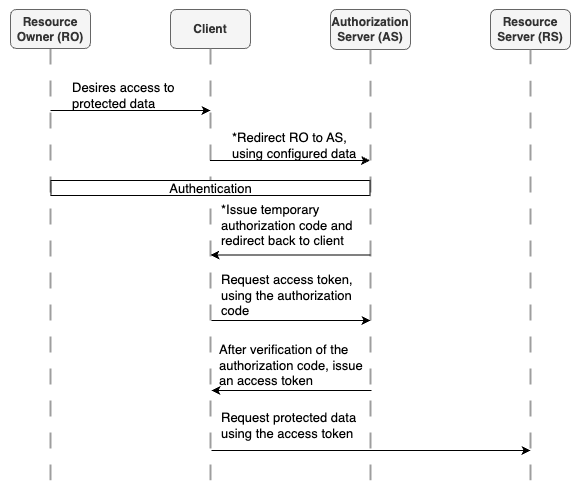
\includegraphics[width=0.75\textwidth]{pic/authorization_code_grant.png}
	\unitlength=0.75mm
	\special{em:linewidth 0.4pt}
	\linethickness{0.4pt}
	\caption{Authorization Code Grant without any extensions}
	\label{fig:auth_code_grant}
\end{figure}

\subsubsection{Implicit Grant}
The Implicit Grant was introduced at a time when there were no mechanisms like Cross-Origin resource sharing implemented in browsers, to share content from different domains. It is a predecessor of the authorization code flow and works similarly with the difference of leaving out the exchanging of the authorization code step as visualized in figure \ref{fig:implicit_grant}. Instead, the access token is sent via the front channel directly from the authorization server to the client. This leaves open more attack vectors for example by utilizing the browser history or by simplifying access token injection \cite{lodderstedt2020oauth}. The Implicit Grant is officially deprecated but still has its relevance, as it is still offered by 37\% of common identity providers \cite{philippaerts2022oauch}.

\begin{figure}[ht]
	\sffamily\footnotesize
	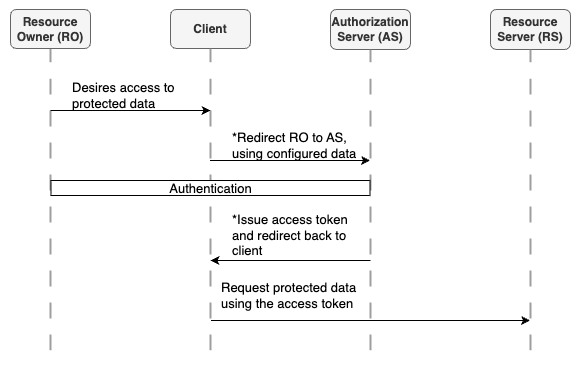
\includegraphics[width=0.75\textwidth]{pic/implicit_grant.png}
	\unitlength=0.75mm
	\special{em:linewidth 0.4pt}
	\linethickness{0.4pt}
	\caption{Implicit Grant}
	\label{fig:implicit_grant}
\end{figure}

\subsubsection{Resource Owner Password Credentials Grant}
This grant type is special in the way that the client is providing its authentication credentials for the authorization provider to the resource provider instead, as illustrated in figure \ref{fig:resource_owner_password_credentials_grant}. The resource provider then uses the credentials to retrieve authorization from the authorization provider. This grant type is only feasible for the scenario, that the resource provider is trusted completely \cite{hardt2012rfc}.

\begin{figure}[H]
	\sffamily\footnotesize
	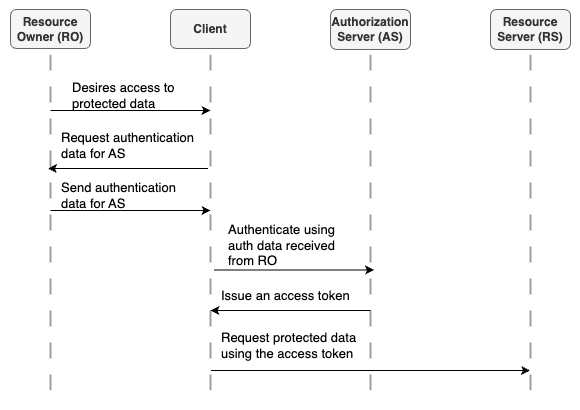
\includegraphics[width=0.75\textwidth]{pic/resource_owner_password_credentials_grant.png}
	\unitlength=0.75mm
	\special{em:linewidth 0.4pt}
	\linethickness{0.4pt}
	\caption{Resource Owner Password Credentials Grant}
	\label{fig:resource_owner_password_credentials_grant}
\end{figure}
	

\subsubsection{Client Credentials Grant}
The client credentials grant is designed to only be used by confidential clients interacting with each other. This means the clients have the ability to securely store a secret, which is only accessible by themselves. A common use case for this scenario would be machine-to-machine interactions. This grant type is meant for clients to access their own resources, which is verified by the possession of the client secret. An example of such a scenario is micro-service architectures. As depicted in figure \ref{fig:client_credentials_grant} the client authenticates at the authorization server with its client secret and receives an access token, to authenticate at the resource provider. This means that the resource provider does not need to verify client secrets, but instead only needs the capability to verify access tokens. This fact is useful for practical reasons, as a resource provider could reuse the implementation of access tokens for other grant types it is offering. \cite{hardt2012rfc}

\begin{figure}[H]
	\sffamily\footnotesize
	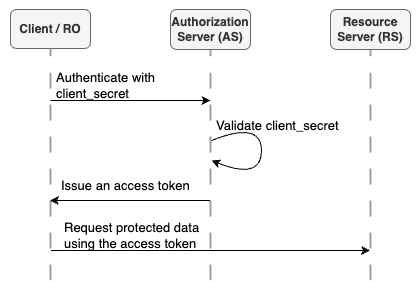
\includegraphics[width=0.6\textwidth]{pic/client_credentials_grant.png}
	\unitlength=0.75mm
	\special{em:linewidth 0.4pt}
	\linethickness{0.4pt}
	\caption{Client Credentials Grant}
	\label{fig:client_credentials_grant}
\end{figure}

\subsubsection{Device Authorization Grant}
Introduced in RFC8628 the device authorization grant, illustrated in Figure \ref{fig:device_authorization_grant} is meant to be used for
devices, that lack a user agent like a web browser or do not offer a convenient
way of entering text \cite{denniss2019oauth}. In this grant type the client is
not mainly interacting through a user agent like a web browser anymore, but instead is using a device authorization endpoint at authorization provider directly to initiate an authorization request. The client, then instructs the user to open a webpage on a secondary device to complete the authorization process using a displayed code for verification of the session. This OAuth flow still requires the involved devices to use HTTP for communication.

\begin{figure}[H]
	\sffamily\footnotesize
	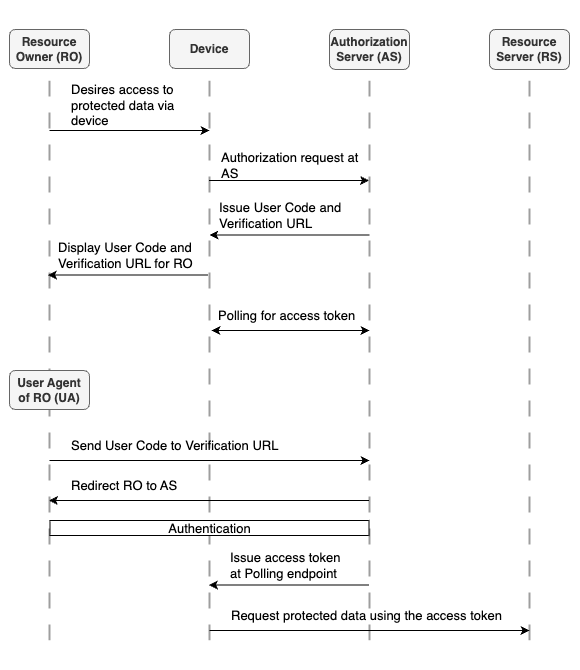
\includegraphics[width=0.75\textwidth]{pic/device_authorization_grant.png}
	\unitlength=0.75mm
	\special{em:linewidth 0.4pt}
	\linethickness{0.4pt}
	\caption{Device Authorization Grant}
	\label{fig:device_authorization_grant}
\end{figure}

\subsubsection{Other grant types}
For the purpose of thoroughness, it is to mention, that there are several more grant types, which got introduced to the OAuth standard over time. These additional grant types are listed below, but are out of scope for this work and are not getting explained further: 

\begin{enumerate}
	\item Refresh Token Grant
	\item JWT Bearer Grant
	\item UMA Grant
	\item SAML 2.0 Bearer Grant
	\item Token Exchange Grant
\end{enumerate}

\subsection{Open ID Connect}
Open ID Connect (OIDC) is a layer on top of OAuth 2.0, introduced in 2014 by a combination of researchers and companies like Google, Microsoft and Salesforce, which form the OpenID group. The main focus of Open ID Connect is authentication, which means identifying a user. The authorization of the identified user is a secondary purpose. OIDC flows use a particular OAuth scope (an additional message, besides \emph{state}, \emph{client\_id}, and similar), which is called \emph{openid}. OIDC also utilizes an extra token, the \emph{ID} token, which is a JWT token containing the identifying information about the user, which are called claims. The claims can be used to retrieve more information about the user at the OpenID provider, or the information can be directly part of the initial \emph{ID} token, so OpenID adds the authentication to the already provided Authorization capability of OAuth. For OIDC, the same grants are used as for OAuth, but in the context of OIDC, they are often referred to as flows \cite{li2016analysing} \cite{sakimura2014openid}.

\subsection{The Future: OAuth 2.1}
OAuth 2.1 will be the next version of OAuth. There is currently one draft available at the IETF \cite{ietf-oauth-v2-1-09}. The main intent of this draft is to consolidate the various extensions to OAuth introduced in the last years. It simplifies the core document for OAuth 2.0 and omits outdated features because of new browser capabilities, which were introduced over the last years and allow for more secure interactions. Below is a list of significant changes:
\begin{enumerate}
	\item The Implicit Grant gets omitted
	\item The Resource Owner Password Credentials Grant gets omitted
	\item PKCE is required for the Authorization Code Grant
	\item Redirect URIs must be compared with exact string matching, so pattern matching is completely disallowed
	\item Access tokens must not be transported in a Request-URI in any case (which also makes the Implicit Grant impossible
\end{enumerate}

In conclusion, the draft for OAuth 2.1 picks valuable features of existing standards for OAuth to require them and omits outdated features, intending, on the one hand, to simplify the OAuth landscape and, on the other hand, get rid of insecure features of the past.

\section{Intrusion Detection System}
An intrusion is any malicious behavior with the intention to damage or take control of an information system. All primary protection goals of information security, like confidentiality, integrity and availability, can be the target of an intrusion. A method to harden systems against intrusions is utilizing intrusion detection systems (IDS), which monitor all traffic, events or actions of a system to detect when malicious actions are executed so the system's owner, the administrator or the system itself can take immediate action on intrusion attempts. If the intrusion detection system takes action to prevent intrusions, it is called an \emph{Intrusion Detection and Prevention System (IDPS)} \cite{scarfone2010intrusion}. There are several taxonomies for intrusion detection system types. For example, Liao et al. \cite{Liao2013IntrusionDS} categorized IDS into five categories: Statistics-based, Pattern-based, Rule-based, State-based, and Heuristic-based, referring to the methodology of detection the IDS is using. \cite{khraisat2019survey} build on top of that approach to further specify an overall taxonomy for IDS. The definition of Intrusion detection systems is based on the taxonomy summarized by these researchers.

\subsection{Distinction by input data}
Generally, when categorizing Intrusion Detection Systems by environment or input data, there are two types to distinguish them. 
\emph{Host-based Intrusion Detection Systems (HIDS)} and \emph{Network-based Intrusion Detection Systems (NIDS)}.
\subsubsection{Host-based Intrusion Detection System}
HIDS monitor all data concerning a host system, like operating system events, host firewall logs or application-specific logs. They can detect specific attacks on the system level without the usage of network logs.
\subsubsection{Network Intrusion Detection System (NIDS)}
NIDS monitor network traffic, which is acquired by packet capture tools and other network data sources. One challenge of Network Intrusion Detection Systems is often the large amount of data that needs to be analyzed in high-bandwidth networks, which demands high computing capabilities.

\subsection{Distinction by detection characteristic}
When distinguishing types of intrusion detection systems by the way they operate, there are two categories: Signature-based (SIDS) and Anomaly-based (AIDS). These categories can then be combined with the above categories, which are distinguished by input data, depending on the context.

\subsubsection{Signature-based Intrusion Detection System}
Signature-based IDS utilize databases of fingerprints of already known attacks. These databases are called knowledge databases. A fingerprint could be, for example, a hash value of an executable malware file. A HIDS could compare any file an operating system executes against the knowledge database to detect the specific malware. The same concept also works for NIDS, e.g., when scanning mail attachments transferred via SMTP. The main advantage of SIDS is that they rarely produce false positive alerts when identifying intrusions. Their downside is that they cannot detect unknown attacks.

\subsubsection{Anomaly-based Intrusion Detection System}
The core concept for Anomaly-based IDS is to differentiate between usual and unusual behavior. Unusual behavior is identified as an intrusion. There is a variety of techniques that AIDS can use to achieve the goal of differentiating typical and malicious behavior. One possibility is creating a statistical model over the data and filtering out events with a low probability. 
Another approach is to use machine learning techniques. Unsupervised learning methods, like clustering, on the one hand, are very similar to the statistical approach because the goal is again to sort out rare occurrences in small clusters. Supervised learning methods, on the other hand, create a model of usual behavior in a training phase with labeled data to test any new input of unknown data if it is classified as malicious. 
An additional way for Anomaly-based IDS is the knowledge-based method. With this method, knowledge is applied to the detection in the form of rules to identify any behavior that breaks those rules as an intrusion. These rules can stem from knowledge about a network protocol or any other system behavior.

\subsection{zeek IDS}
One example of an implementation of an intrusion detection system is called \emph{zeek}.\emph{Zeek} formerly known as \emph{bro}, as a reference to George Orwell's 1984 as a ``reminder that monitoring comes hand in hand with the potential for privacy violations'' \cite{zeek2023} is an open source network intrusion detection system. The first version of \emph{bro} was released in 1995 by the Lawrence Berkeley National Laboratory. In 2018, the project was renamed to \emph{zeek}. The system is often used for network security monitoring to detect and analyze suspicious behavior in network traffic. Its architecture consists of two major components, as displayed in Figure \ref{fig:zeek_architecture}. The first component is the \emph{event engine}, which refines the incoming network traffic into higher-level events without doing any analysis. It processes the traffic through different subcomponents, identifying protocols, file types, and, e.g. TCP connections at the link layer. The second component is the \emph{policy script interpreter}, which runs different event handlers to analyze the events. These event handlers are built in their own scripting language, but adapters to popular programming languages also exist and are applied in this work.

\begin{figure}[H]
	\sffamily\footnotesize
	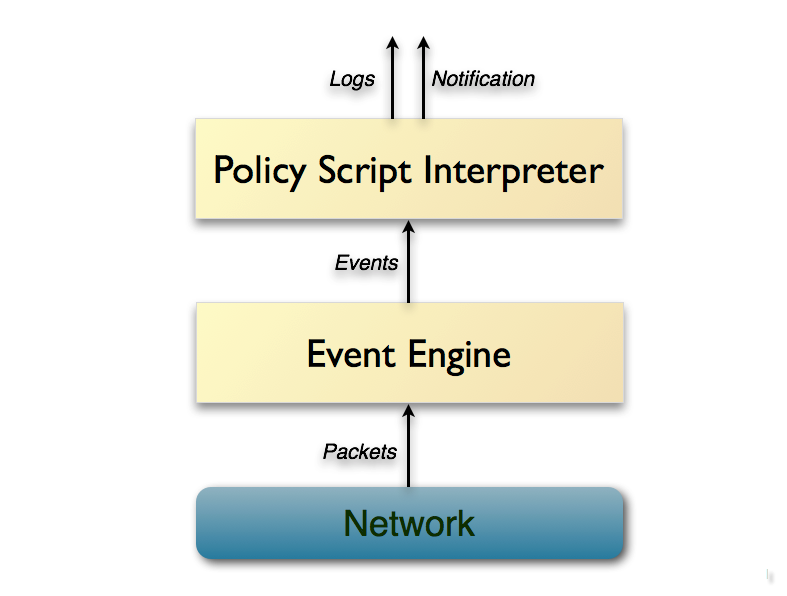
\includegraphics[width=0.75\textwidth]{pic/zeek_architecture.png}
	\unitlength=0.75mm
	\special{em:linewidth 0.4pt}
	\linethickness{0.4pt}
	\caption{Architecture of zeek \cite{zeek2023}}
	\label{fig:zeek_architecture}
\end{figure}

\section{Algorithms}
The algorithms applied in the experimental part of this work serve different purposes in the experiment chain described in Chapter \ref{chap:experimental_analysis}. These algorithms are essential for following along with the experimental approach. Therefore, this section starts by describing the technique for encoding the textual network data to numerical data. It follows up by illustrating the inner workings of two clustering algorithms applied to the encoded data at the end of the experiments.


\subsection{Word2Vec}
\emph{Word2Vec} introduced in 2013 by Mikolov et al. is a technique in natural language processing to convert words into embeddings. An embedding is a vector carrying a semantic to represent a word as a numerical value to enable the usage of words in algorithms requiring numerical inputs. In the case of \emph{Word2Vec}, the idea is that words hold similarities based on their surrounding words in a text corpus. This concept leads to words, which often stand close together in a text, receiving vectors that point in a similar direction. Two models are employed by \emph{word2vec}, the \emph{Continuous Bag of words (CBOW)} model and the \emph{Skip-Gram} model. Both models have in common that they apply supervised learning techniques by training a neural network to predict relationships in text corpora. In both cases, the goal is to use the weights of the hidden layer after training as word embeddings instead of utilizing the neural networks for any predictions \cite{mikolov2013efficient} \cite{rong2014word2vec}.

\subsubsection{Continuous Bag of Words (CBOW)}
The continuous bag of words model trains a neural network that predicts the word in the middle based on its surrounding words. An important hyperparameter for CBOW and Skip-Gram is the window size, which describes how many words surrounding a word are considered context. 
During training, the network receives combined one-hot-encoded vectors of surrounding words (e.g., averaging or summing them) in a tuple with the corresponding target word. When the training is completed at inference, the model gets context words as input and outputs a vector of probabilities for the predicted target word. But as mentioned above, the goal of word2vec is to extract word embeddings, which are the weights of the hidden layer of the neural network.

\subsubsection{Skip-Gram}
The skip-gram model uses the reverse strategy compared to the CBOW model. Instead of predicting a word by its surroundings, it trains a neural network that tries to predict the surroundings of a word. At training, the neural network receives word tuples of single context words and their corresponding target words one-hot-encoded. After fitting the network during inference, the model receives a one-hot-encoded word as input and produces a probability distribution over the vocabulary, which stands for the probability of a word being a surrounding word for the input. Again, in the case of word2vec, this supervised learning approach is only applied to retrieve the weights of the hidden layer as word embeddings, as word2vec is used for non-labeled, unsupervised data. In their research, Mikolov et al. state that \emph{skip-gram} is feasible for small data sets and even considers rare occurrences of words well. In contrast, \emph{CBOW} is faster in training with large datasets and better at capturing the semantics of high-frequency words. 

\subsection{k-means Clustering}
In the field of data analysis, finding patterns and anomalies in data sets is a ubiquitous challenge. Grouping data into different clusters can be an approach to reveal useful features or meanings from the data. One common technique for clustering is k-means clustering. There are different flavors of k-means algorithms, but one of the most common k-means algorithms and the one applied in this work is Lloyd's k-means algorithm \cite{wilkin2007kmeans}. 

\subsubsection{Lloyd's k-means clustering}
The general goal of the algorithm is to group data by similar features into a fixed amount of clusters. The algorithm achieves this by finding $k$ \emph{centroids} $\mu_1, \mu_2 ... \mu_k \in \mathbb{R}$, which are cluster defining centers. The clusters are based on the centroids in the way that every point $x$ of the n-dimensional dataset ${x_1 ... x_m}$ gets assigned to the centroid with the lowest Euclidean distance. In order to find the centroids, the algorithm's approach is an iterative process described in Algorithm \ref{alg:kmeans}. In the beginning, $k$ (defined by the number of clusters) random centroids are chosen. Then, the clusters are created by calculating the minimum Euclidean distance from every point of the dataset to the centroids: $\arg\min_j \|x_i - \mu_j\|^2$. In the next step, the centroids are recalculated by finding the points in the center of the clusters: $\mu_j = \ \frac {1}{|\mu_j|} \sum_{x_i \in \mu_j} x_i$. The two steps of creating the clusters based on the centroids and calculating the center point of the new clusters are repeated until the centroids converge or a definition for a fixed amount of iterations is given \cite{piech2013kmeans} \cite{lloyd1982kmeans}. In the end, every point of the dataset belongs to the cluster centroid with the minimum Euclidean distance.


\begin{algorithm}
	\caption{Lloyd's K-Means Algorithm}
	\label{alg:kmeans}
	\begin{algorithmic}
		\State \textbf{Input:} Data set $X = {x_1 \ldots x_m}$, number of clusters $k$
		\State \textbf{Output:} Cluster centroids $\{\mu_1, \mu_2, \ldots, \mu_k\}$
		\State Randomly choose $k$ centroids ${\mu_1 \ldots \mu_k}$ 
		\Repeat
		\For{each data point $x_i$}
			\State Assign $x_i$ to the cluster with the nearest centroid: $\mu_i = \arg\min_j \|x_i - \mu_j\|^2$
		\EndFor
		\For{each cluster $j$}
			\State Calculate new centroid $\mu_j$ as the center of all points assigned to cluster $j$ for every cluster: $\mu_j = \frac{1}{|\mu_j|} \sum_{x_i \in \mu_j} x_i$
		\EndFor
		\Until{New centroids don't change anymore or a fixed number of iterations was given}
	\end{algorithmic}
\end{algorithm}

\subsection{Self-Organizing Maps}
\label{subsec:self-organizing_maps}
A Self-Organizing Map (SOM) is an unsupervised machine-learning algorithm that aims to reduce the dimensions of high-dimensional data. SOMs were introduced in 1990 by the Finnish engineer and senior member of the IEEE Teuvo Kohonen. As described in the initial publication, Self-Organizing Maps not only help with dimension reduction but also can discover semantic relationships in sentences \cite{Kohonen1990}.
This aspect, in particular, is one reason the algorithm is applied in fields other than data visualization as well, like natural language processing and intrusion detection \cite{qu2021survey}. The following explanation is based on the original publication by Kohonen. At its core, a Self-Organizing Map is based on an artificial neural network that is trained using competitive learning. The network's input layer usually has many more dimensions than the output layer, which aligns with the algorithm's goal to reduce the dimensions of data. Then, there is an inner layer called the Kohonen Layer, a grid of neurons with the desired output's dimensions. This layer of neurons gets initialized at random in the beginning. The training process now works as follows:

\begin{enumerate}
	\item An input vector of the sample high-dimensional data gets randomly chosen. The neuron in the Kohonen layer, whose weight is most similar to the input vector, gets chosen by calculating the Euclidean distance: $$D(w, x) = \sqrt{\sum_{i=1}^{N} (w_i - x_i)^2}$$ for weight vector $w$, input vector $x$ for $N$ dimensions. The weight vector, which is chosen this way, is called the \emph{winner} or the \emph{Best Matching Unit (BMU)}.
	\item A neighborhood function gets applied to the BMU, influencing the weights of neighboring neurons. The neighborhood function is most often a Gaussian decay function: $$h(r, t) = \exp\left(-\frac{2\sigma^2(t)}{\|r\|^2}\right)$$ where $\|r\|^2$ is the Euclidean distance between the BMU and the neighbor, $t$ is the time (or iteration amount), which has passed and $\sigma^2(t)$ is the neighborhood radius, which decreases over time. This formula leads neurons near the BMU to be updated more heavily in the early stages of the training.
	\item The weights of the Kohonen layer are updated for multiple iterations to resemble the input vectors in the end. The output is the weights of the Kohonen layer, which have been reduced to the desired lower dimension.
\end{enumerate}
